
\section{Исследование и описание решения задачи}
\label{sec:survey}
\subsection{Стратегия разработки}
\label{subsec:develop_strat}

\begin{table}[h]
\centering
\begin{tabular}{|c|c|c|}
\hline
\begin{tabular}[c]{@{}c@{}}Название \\ нейронной\\ сети\end{tabular} & Ссылка на статью         \\ \hline
\textbf{Задача классификации:}                                       &                          \\ \hline
Resnet                                                               & \cite{resnet_2015}       \\ \hline
EfficientNet                                                         & \cite{efficientnet_2019} \\ \hline
Resnext                                                              & \cite{resnext_2016}      \\ \hline
SimpleViT                                                            & \cite{simplevit_2022}    \\ \hline
Swin Transformer V2                                                  & \cite{swin_2021}         \\ \hline
DINOv2                                                               & \cite{dinov2_2024}       \\ \hline
CLIP                                                                 & \cite{clip_2021}         \\ \hline
MoViNet                                                              & \cite{movinet_2021}      \\ \hline
\textbf{Задача детекции:}                                            &                          \\ \hline
YOLOv11                                                              & \cite{yolov11_2024}      \\ \hline
\textbf{Задача сегментации:}                                         &                          \\ \hline
UNET/UNET+/UNET++                                                    & \cite{unet_2015}         \\ \hline
SAM/SAM2                                                             & \cite{sam2_2024}         \\ \hline
\end{tabular}
\caption{Список моделей для тестирования}
\label{tbl:models}
\end{table}

Разработка полнофункциональных аналогов библиотек cuBLAS и cuDNN представляет собой
обширную инженерную задачу, требующую четкого определения приоритетов. Выбор фокуса разработка сильно обусловлен
спецификой целевой платформы. Например, на встраиваемых системах Nvidia Jetson задачи вывода (inference) составляют основной
рабочий сценарий. Разрабатываемый GPGPU ускоритель предполагает схожие сценарии работы, поэтому основным приоритетом является
inference-режим.

Учитывая, что библиотеки cuBLAS и cuDNN преимущественно используются через высокоуровневые фреймворки (PyTorch, TensorFlow),
критически важными становятся бесшовная интеграция с существующими API, соответствие ожидаемому поведению в реальных сценариях
и стабильность работы в составе сложных задач машинного обучения. В качестве референсной платформы для верификации предлагается
использовать PyTorch, что обеспечивает:
\begin{itemize}
\item Доступ к широкому спектру готовых моделей (ResNet, BERT, YOLO)
\item Тестовое покрытие на реальных задачах
\item Возможность интеграции с инструментами профилирования Nvidia Nsight \cite{nsight_systems_2025}
\end{itemize}
Для систематизации процесса разработки аналогов библиотек cuBLAS и cuDNN был проведен анализ функций,
наиболее востребованных при работе с нейронными сетями в режиме вывода (inference).
Принято решение о фиксации набора эталонных моделей, которые удовлетворяют следующим критериям отбора:
\begin{itemize}
    \item Широкая распространенность в промышленных решениях
    \item Соответствие требованием заказчика GPGPU ускорителя
\end{itemize}

Отобранные модели работали в режиме вывода и представлены в табл. \ref{tbl:models}. После фиксации моделей
были зафиксированы все интерфейсы библиотек cuBLAS и cuDNN c помощью утилиты трассирования \textit{ltrace}.
Анализ показал, что во всех представленных сетях больше всего задействованы следующие вызовы:
\begin{itemize}
   \item \textbf{cuBLAS}
    \begin{itemize}
        \item \texttt{cublasLtMatmul} — общее матричное умножение (GEMM — general matrix multiplication)
    \end{itemize}

    \item \textbf{cuDNN}
    \begin{itemize}
        \item \texttt{cudnnConvolutionForward} — прямая свертка тензора (обычно 4-мерного в формате NCHW или NHWC)
        \item \texttt{cudnnBatchNormalizationForwardInference} — пакетная нормализация тензора
    \end{itemize}
\end{itemize}

\subsection{Схема запуска на симуляторе gem5}

\begin{figure}
    \centering
    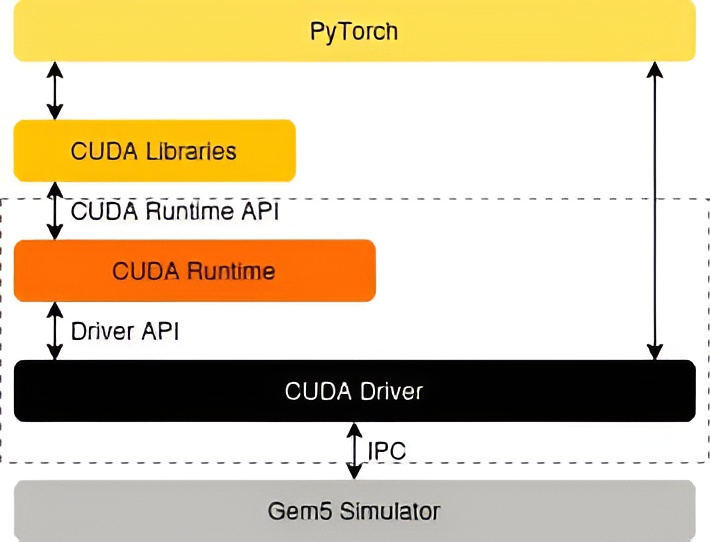
\includegraphics[scale=0.4]{src/images/launch_scheme.jpeg}
    \caption{Запуск приложения на функциональном/потактовом симуляторе}
    \label{fig:launch_scheme}
\end{figure}

Представленные нейронные сети должны быть запущены на функциональном и потактовом симуляторе GPGPU, поддерживающего модель CUDA.
На рисунке \ref{fig:launch_scheme} представлена архитектурная схема выполнения нейронных сетей из таблицы \ref{tbl:models}
на функциональном и потактовом симуляторе. Как следует из схемы, процесс выполнения в PyTorch включает
многоуровневую систему вызовов.

При запуске нейронной сети фреймворк PyTorch обращается к функциям библиотек cuBLAS и cuDNN, которые содержат реализации вычислительных
алгоритмов в виде CUDA kernel. При запуске CUDA kernel вызываются функции библиотеки времени выполнения (например, \texttt{cudaLaunchKernel})
и функции драйвера устройства.

Библиотека времени выполнения предоставляет высокоуровневый API для управления вычислительным устройством.
Драйвер устройства обеспечивает непосредственное взаимодействие с аппаратными ресурсами
через набор низкоуровневых интерфейсов. Библиотека времени выполнения использует низкоуровневые интерфейсы драйвера
для реализации своего функционала.

В предложенной архитектуре драйвер устройства через механизм межпроцессорного взаимодействия (IPC) передает вычислительные задачи на
симулятор, который эмулирует выполнение соответствующих CUDA kernel. Для преобразования исходного кода CUDA в исполняемый формат
используется специализированный компилятор на базе инфраструктуры LLVM \cite{llvm_project_2025}, обеспечивающий оптимизацию под целевую платформу.

\subsection{Методология тестирования}
При разработке GPGPU критически важным является верификация результатов вычислений. При этом разработка значительно упрощается
при наличии эталонной реализации. В качестве эталонной платформы выбраны устройства компании Nvidia, что обусловлен их доминирующим
положение на рынке ускорителей для машинного обучения.

При тестировании \textit{функциональной} корректности библиотек cuBLAS и cuDNN архитектурные особенности реализации (такие как конвейерная
обработка команд или организация иерархии памяти) не являются определяющими факторами. Это позволяет существенно оптимизировать процесс
тестирования, разделив его на два параллельных направления. Основной объем тестирования выполняется на реальных устройствах NVIDIA Jetson,
что имеет следующие ключевых преимущества:
\begin{itemize}
    \item Высокая скорость выполнения тестовых прогонов по сравнению с симулятором
    \item Возможность быстрых итераций при разработке
    \item Проверка библиотек в реальных условиях
\end{itemize}
Параллельно осуществляется тестирование на симуляторе, которое фокусируется на осуществлении соответствия
семантики исполнения инструкции, описанными в документе разрабатываемого ускорителя.

Как уже отмечалось были зафиксированы три ключевых интерфейса: \texttt{cublasLtMatmul}, \texttt{cudnnConvolutionForward},
\texttt{cudnnBatchNormalizationForwardInference}, которые используются нейронными сетями из табл. \ref{tbl:models}. Помимо этого
были сняты все параметры интерфейсов, включая:
\begin{itemize}
    \item Размерности тензоров
    \item Тип данных и формат хранения
    \item Параметры операции, такие как шаг свертки
    \item Дополнительные параметры, регулирующие выбор алгоритмов
\end{itemize}
Далее были построены тесты, которые сравнивали эталонную реализацию cuDNN и cuBLAS с разрабатываемыми аналогами в описанных сценариях
с необходимой точностью.

\subsection{Методология оценки производительности}
\label{subsec:perf_eval}
В отличие от функционального тестирования, анализ производительности требует более детального и системного подхода.
Разработка конкурентоспособного GPGPU-ускорителя предполагает достижение высокой эффективности при выполнении промышленных
задач, что обуславливает необходимость комплексной методики измерений.

Основным инструментом для точной оценки временных характеристик разрабатываемой архитектуры служит тактовый (cycle-accurate) симулятор
на базе платформы gem5. Данный инструментарий позволяет получить детальную информацию о ключевых метриках производительности, такие как
количество тактов, статистика работы иерархии памяти, загрузку вычислительных блоков.

Однако необходимо отметить, что потактовые симуляторы характеризуются чрезвычайно высокой вычислительной стоимостью,
что существенно ограничивает их применение для оперативной оценки производительности в процессе разработки.

Учитывая архитектурную близость разрабатываемого решения к GPU NVIDIA, была принята методика кросс-валидации
производительности на реальных устройствах серии Jetson Xavier. Данный подход основан на следующих допущениях:
\begin{itemize}
    \item Оптимизированные для архитектуры NVIDIA задачи демонстрируют сопоставимую эффективность на разрабатываемом ускорителе
    \item Относительные показатели производительности сохраняются
    \item Принцип написания высокоэффективного CUDA-кода коррелируют между платформами
\end{itemize}

Таким образом, в данной работе большее внимание уделена анализу производительности и функциональной корректности
на реальных графических процессора Nvidia.

\subsection{Реализация операция \texttt{cublasLtMatmul}}
% \subsubsection{Описание возможностей}
Операция \texttt{cublasLtMatmul} реализует обобщенное матричное умножение с возможностью дополнительных преобразований.
Формально операция определяется следующим образом:

Пусть заданы:
\begin{itemize}
    \item $\mathbf{A} \in \mathbb{F}^{M \times K}$ - входная матрица
    \item $\mathbf{B} \in \mathbb{F}^{K \times N}$ - входная матрица
    \item $\mathbf{C} \in \mathbb{F}^{M \times N}$ - дополнительная матрица
    \item $\mathbf{D} \in \mathbb{F}^{M \times N}$ - результирующая матрица
\end{itemize}

Тогда результат вычисляется по формуле:
\begin{equation}
\mathbf{D} = \text{epilogue}\left(\alpha \cdot \text{op}(\mathbf{A}) \cdot \text{op}(\mathbf{B}) + \beta \cdot \text{op}(\mathbf{C})\right)
\end{equation}

где:
\begin{itemize}
    \item $\text{op}(\cdot)$ - оператор преобразования матрицы (тождественный, транспонирование или эрмитово сопряжение)
    \item $\text{epilogue}(\cdot)$ - постобработка результата (например, функция активации ReLU)
    \item $\alpha, \beta \in \mathbb{F}$ - скалярные коэффициенты
    \item $\mathbb{F}$ - некоторое поле, обычно $\mathbb{R}$ или $\mathbb{C}$
\end{itemize}

Размерности матриц должны удовлетворять условию согласованности: если $\text{op}(\mathbf{A})$ имеет размер
$m \times k$, а $\text{op}(\mathbf{B})$ - размер $k \times n$, то $\text{op}(\mathbf{C})$ должен иметь размер $m \times n$.

Среди возможных функций постобработки часто применяется \textit{вектор смещений}.
В контексте матричных операций под вектором смещений (bias vector) понимается операция вида:
\begin{equation}
D_{i,j} = \left(\alpha \cdot (\mathbf{A}\mathbf{B})_{i,j} + \beta \cdot C_{i,j}\right) + b_j \quad \text{для} \quad i=1,\ldots,M; \ j=1,\ldots,N
\end{equation}

где:
\begin{itemize}
    \item $b_j$ - $j$-тый элемент вектора смещений
    \item Сложение с вектором выполняется путем его неявного расширения (broadcasting) по строкам
\end{itemize}

Помимо базовой реализации матричного умножения, операция \texttt{cublasLtMatmul} поддерживает возможность пакетной обработки
(\textit{batched GEMM}). Формально операция описывается как:
\begin{equation}
\mathbf{D}_i = \text{epilogue}\left(\alpha \cdot \text{op}(\mathbf{A}_i) \cdot \text{op}(\mathbf{B}_i) + \beta \cdot \text{op}(\mathbf{C}_i)\right), \quad i = 1,\ldots,N
\end{equation}
Опять же матрицы должны удовлетворять условию согласованности размеров.

% \subsubsection{Тестовая выборка}
\begin{table}[h]
\centering
\begin{tabular}{|l|c|c|r|}
\hline
\multicolumn{1}{|c|}{\textbf{Тип данных}} & \textbf{Батчинг} & \textbf{Эпилог} & \textbf{Кол-во тестов} \\ \hline
float32 & Нет & Вектор смещений & 29 \\ \hline
float32 & Да & Нет & 19 \\ \hline
complex32 & Да & Нет & 123 \\ \hline
complex32 & Нет & Нет & 7 \\ \hline
\hline
\multicolumn{3}{|l|}{\textbf{Всего:}} & 178 \\ \hline
\end{tabular}
\caption{Классификация вызовов \texttt{cublasLtMatmul} по типам операций}
\label{tbl:cublas_calls}
\end{table}

В таблице \ref{tbl:cublas_calls} приведены все вызовы операции \texttt{cublasLtMatmul}, которые были зафиксированы по методологии,
описанной в разделе \ref{subsec:develop_strat}. Все вызовы были систематизированы по трем ключевым параметрам:
\begin{itemize}
\item Типу обрабатываемых данных (вещественные или комплексные числа)
\item Наличию пакетной обработки (\textit{batching})
\item Применению дополнительных преобразований (эпилогу)
\end{itemize}

% \subsubsection{Параметры конфигурации GEMM в CUTLASS: влияние на загрузку потоков и производительность}
Анализ возможностей библиотеки CUTLASS показал, что CUTLASS поддерживает необходимый функционал для
реализации операции \texttt{cublasLtMatmul}. В CUTLASS имеется реализации пакетной обработки и операций
с комплексными числами, однако есть ограничения на вектор смещений. На момент написания реализации \texttt{cublasLtMatmul}
CUTLASS не поддерживал одновременное использование матрицы $\mathbf{C}$ и вектора смещений.

В отличие от библиотеки cuBLAS, которая автоматически выбирает оптимальные алгоритмы для заданных параметров задачи,
CUTLASS требует явного указания вычислительных параметров через шаблонные классы.
Для оценки производительности использовалась платформа NVIDIA Jetson Xavier, архитектурные характеристики которой наиболее
близки к разрабатываемому GPGPU-ускорителю.

Ключевым параметром, определяющим производительность на данной платформе, являются размеры подматриц, обрабатываемых отдельными
блоками и варпами. В CUTLASS 2.x эти параметры задаются шаблонным классом \texttt{cutlass::GemmShape<\~{M}, \~{N}, \~{K}>}, где для матрицы
$\mathbf{A}$ выделяется подматрица размера $\tilde{M} \times \tilde{K}$, для $\mathbf{B}$ - $\tilde{K} \times \tilde{N}$, а для результирующей
матрицы $\mathbf{D}$ - $\tilde{M} \times \tilde{N}$.

Конкретный пример с размерами подматриц для блока \texttt{cutlass::GemmShape<128, 64, 8>} определяет следующие характеристики:
\begin{itemize}
    \item Требования к общей памяти:
    \begin{itemize}
        \item Для матрицы $A$: $128 \times 8 \times \text{размер элемента}$
        \item Для матрицы $B$: $64 \times 8 \times \text{размер элемента}$
    \end{itemize}
    \item Область данных, параллельно обрабатываемую одним CUDA-блоком
\end{itemize}

\begin{figure}[h]
    \centering
    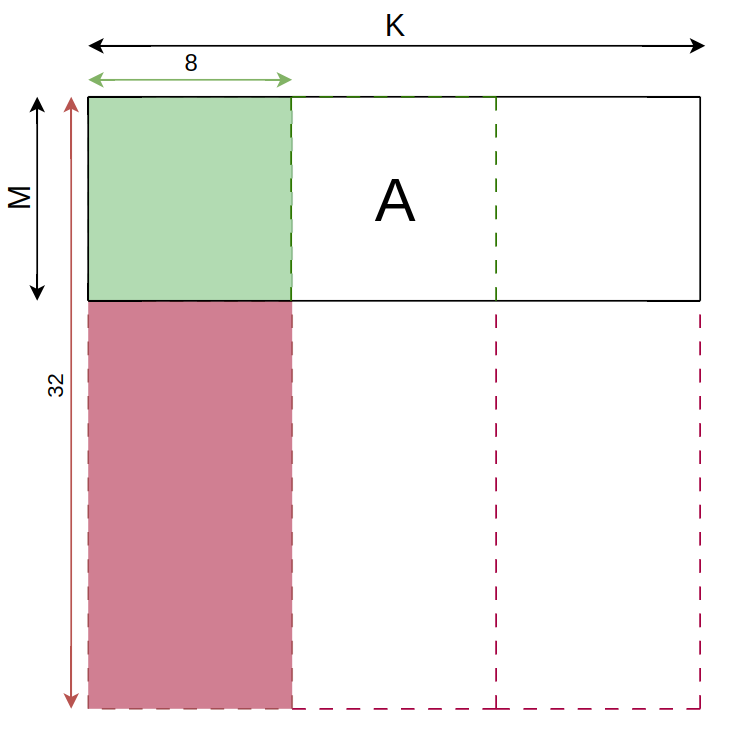
\includegraphics[width=0.8\textwidth]{src/images/block_sizes_no_grid.png}
    \caption{Пример неоптимального выбора параметров ($\tilde{M}=32$ для $M<32$): красным выделены простаивающие потоки}
    \label{fig:block_sizes}
\end{figure}

В CUTLASS для утилизирования тензорных инструкций [x] также располагает размерами подматрица, обрабатываемых отдельными потоками.
В рассматриваемой реализации каждый поток обрабатывает один элемент матрицы, что задаётся параметром \texttt{cutlass::GemmShape<1, 1, 1>}.
Такой выбор связан с тем, что в тестах отобраны вызовы не предполагающие использование тензорных инструкций.
В совокупности с размерами подматриц, обрабатываемых отдельными варпами, можно однозначно определить количество варпов в блоке и соотвественно
количество потоков в блоке.

Выбор оптимальных значений $\tilde{M}$, $\tilde{N}$ и $\tilde{K}$ может учитывать:
\begin{itemize}
    \item Размера исходных матриц
    \item Ограничения по размеру общей памяти
    \item Особенности планирования варпа на целевой архитектуре
\end{itemize}

Для определения оптимальных значений $\tilde{M}$ и $\tilde{N}$ предложен простой и эффективный метод,
основанный на анализе размеров исходных матриц. Алгоритм для $\tilde{M}$ (аналогично для $\tilde{N}$) описывается следующим образом:

Пусть:
\begin{itemize}
    \item $M$ -- размер исходной матрицы по строкам
    \item $L = \{16, 32, 64, 128\}$ -- множество допустимых размеров подматриц (степени двойки)
\end{itemize}

Тогда оптимальное значение $\tilde{M}$ определяется как:
\begin{equation}
\tilde{M} =
\begin{cases}
\max \{ l \in L \mid l \leq M \}, & \text{если } M \geq 16 \\
16, & \text{если } M < 16
\end{cases}
\end{equation}

Как показано на рис. \ref{fig:block_sizes}, выбор $\tilde{M}=32$ для матрицы с $M<32$ приводит к значительному простою потоков (выделены красным).
Предложенный алгоритм позволяет увеличить отношение работающих потоков к простаивающим и обеспечить более высокую загрузку вычислительных блоков.

\begin{figure}[ht]
\centering
\begin{tikzpicture}
\begin{axis}[
    ybar,
    width=0.5\textwidth,
    height=0.6\textwidth,
    bar width=0.5cm,
    ymajorgrids=true,
    ylabel={Производительность относительно cuBLAS},
    ymin=0,
    ymax=1,
    symbolic x coords={CUTLASS, CUTLASS+оптимизация},
    xtick=data,
    nodes near coords,
    nodes near coords align={vertical},
    every node near coord/.append style={font=\small, yshift=5pt},
    axis lines*=left,
    tick label style={font=\small},
    label style={font=\small},
    title style={font=\small, align=center},
    title={Сравнение производительности реализаций \\ интерфейса \texttt{cublasLtMatmul}},
    enlarge x limits=0.4
]

\addplot[fill=blue!30, draw=blue!80] coordinates {
    (CUTLASS, 0.35)
    (CUTLASS+оптимизация, 0.9)
};

\end{axis}
\end{tikzpicture}
\caption{Сравнение производительности разработанного решения с cuBLAS на Jetson Xavier: геометрическое среднее
относительного ускорения до и после применения оптимизации}
\label{fig:cublas_bar}
\end{figure}

Количественная оценка эффективности предложенного подхода представлена на рис. \ref{fig:cublas_bar}. Тестирование проводилось на
платформе Nvidia Jetson Xavier по методологии, описанной в разделе \ref{subsec:perf_eval} с использованием тестовых сценариев из таблицы
\ref{tbl:cublas_calls}.

Результаты показывают, что оптимизированная реализация достигает 90\% производительности эталонной библиотеки cuBLAS, что свидетельствует о высокой
эффективности предложенных решений.

\subsection{Реализация \texttt{cudnnBatchNormalizationForwardInference}}
% \subsubsection{Описание возможностей}
Вызов \texttt{cudnnBatchNormalizationForwardInference} представляет собой пакетную нормализацию.
Пусть задан входной тензор $\mathcal{X} \in \mathbb{R}^{N \times C \times H \times W}$, где:
\begin{itemize}
    \item $N$ -- размер батча
    \item $C$ -- количество каналов
    \item $H \times W$ -- пространственные размерности
\end{itemize}

Пакетная нормализация представляет собой последовательность преобразований входных данных, вычисляемых следующим образом:

\begin{enumerate}
    %\item \textbf{Нормализация по батчу}:
\item Для каждого канала $c \in \{1,...,C\}$ вычисляются статистики:
\begin{align}
\mu_c &= \frac{1}{NHW}\sum_{n=1}^N \sum_{h=1}^H \sum_{w=1}^W \mathcal{X}_{n,c,h,w} \label{eq:batch_mean} \\
\sigma_c^2 &= \frac{1}{NHW}\sum_{n=1}^N \sum_{h=1}^H \sum_{w=1}^W (\mathcal{X}_{n,c,h,w} - \mu_c)^2 \label{eq:batch_var}
\end{align}

% \item \textbf{Нормализующее преобразование}:
\item
\begin{equation}
\hat{\mathcal{X}}_{n,c,h,w} = \frac{\mathcal{X}_{n,c,h,w} - \mu_c}{\sqrt{\sigma_c^2 + \epsilon}} \label{eq:norm_transform}
\end{equation}
где $\epsilon > 0$ -- параметр регуляризации.

% \item \textbf{Аффинное преобразование}:
\item
\begin{equation}
\mathcal{Y}_{n,c,h,w} = \gamma_c \hat{\mathcal{X}}_{n,c,h,w} + \beta_c \label{eq:affine_transform}
\end{equation}
где $\gamma_c, \beta_c \in \mathbb{R}$ -- параметры растяжение и смещения для каждого канала.
\end{enumerate}

% \subsubsection{Архитектура реализации}
Для реализации интерфейса \texttt{cudnnBatchNormalizationForwardInference} разработана оптимизированная CUDA-реализация алгоритма пакетной нормализации.
Ключевым аспектом реализации является стратегия параллелизации вычислений, основанная на двумерной организации сетки (grid) и одномерной организации блоков (blocks).
Сетка потоков имеет размерности $C \times N \times 1$, где $C$ - количество каналов, $N$ - размер батча. Каждый блок в этой сетке соответствует фиксированной паре
(канал $c$, батч $n$) и имеет одномерную структуру из 512 потоков.

Каждый такой блок обрабатывает все пространственные измерения $H \times W$ для назначенной пары (канал, батч). Потоки внутри блока параллельно вычисляют элементы
пространственных измерений, обрабатывая данные с шагом 512 элементов. Формально, поток с индексом $t$ вычисляет элементы:
\[
\{\mathcal{X}_{n,c,h,w} | h = \lfloor \frac{(t + k \cdot 512)}{W} \rfloor, w = (t + k \cdot 512)\mod W \}
\]
где $k = 0,1,2,\dots$ до полного покрытия пространственных измерений $H \times W$.

В данной реализации параметры нормализации ($\gamma_c$, $\beta_c$, $\mu_c$, $\sigma_c^2$) загружаются один раз на весь блок, что минимизирует обращения к глобальной
памяти, приэтом обеспечен объединенный (coalesced) доступ к данным, позволяющий эффективно использовать пропускную способность памяти.

% \subsubsection{Оценка производительности}
Производительность реализации оценивалась на наборе из 45 тестовых сценариев, отобранных согласно методологии, изложенной в разделе \ref{subsec:develop_strat}.
Все тесты проводились исключительно с форматом тензоров NCHW, что обусловлено его статусом стандарта де-факто в экосистеме PyTorch.
Результаты тестирования демонстрируют достижение 99.7\% производительности (геометрическое среднее) относительно эталонной реализации cuDNN,
с вариацией результатов от 78\% до 107\% в отдельных тестовых случаях.

\subsection{Реализация \texttt{cudnnConvolutionForward}}
Операция \texttt{cudnnConvolutionForward} реализует свертку тензоров, формально описываемую выражением \eqref{eq:conv}.
Как отмечено в разделе \ref{subsec:cutlass_review}, библиотека CUTLASS поддерживает алгоритм implicit GEMM для свертки
исключительно в формате NHWC. Однако, учитывая что фреймворк PyTorch использует формат NCHW как основной, было принято
решение реализовать поддержку свёртки в этом формате посредством трёхэтапного преобразования:
\begin{enumerate}
\item Преобразование входных тензоров из формата NCHW в формат NHWC
\item Выполнение свёртки с использованием реализации CUTLASS для формата NHWC
\item Обратное преобразование выходного тензора из формата NHWC в формат NCHW.
\end{enumerate}

Для верификации реализации операции \texttt{cudnnConvolutionForward} использовались вызовы свертки,
систематизированные по размеру фильтра и шагу свертки. Распределение тестовых случаев представлено
в таблице \ref{tbl:conv_test_distribution}:

\begin{table}[h]
\centering
\small
\begin{tabular}{|l|c|c|}
\hline
\textbf{Тип свертки} & \textbf{Количество тестов} & \textbf{Сокращение} \\ \hline
Фильтр 1x1, шаг 1x1 & 108 & k1x1s1 \\ \hline
Фильтр 1x1, шаг 2x2 & 9 & k1x1s2 \\ \hline
Фильтр 3x3, шаг 1x1 & 47 & k3x3s1 \\ \hline
Фильтр 3x3, шаг 2x2 & 20 & k3x3s2 \\ \hline
Фильтр 4x4, шаг 4x4 & 1 & k4x4s4 \\ \hline
Фильтр 5x5, шаг 1x1 & 1 & k5x5s1 \\ \hline
Фильтр 7x7, шаг 2x2 & 3 & k7x7s2 \\ \hline
Фильтр 7x7, шаг 4x4 & 1 & k7x7s4 \\ \hline
Фильтр 1xN & 6 & k1xN \\ \hline
Фильтр Nx1 & 51 & kNx1 \\ \hline
Фильтр >=10x10 & 2 & k>=10 \\ \hline
\hline
\multicolumn{1}{|l|}{\textbf{Всего}} & 249 & Overall \\ \hline
\end{tabular}
\caption{Распределение тестовых сценариев свертки по типам операций}
\label{tbl:conv_test_distribution}
\end{table}

\begin{figure}[htbp]
\centering
\begin{adjustbox}{max width=\textwidth}
\begin{tikzpicture}
\begin{axis}[
    ybar=0pt,
    bar width=10pt,
    width=15cm,
    height=8cm,
    enlarge x limits=0.15,
    ylabel={Производительность относительно cuDNN},
    xlabel={Тип свертки},
    symbolic x coords={
        k1x1s1x1, k1x1s2x2, k3x3s1x1, k3x3s2x2,
        k4x4s4x4, k5x5s1x1, k7x7s2x2, k7x7s4x4,
        k1xN, kNx1, k>=10, overall
    },
    xtick=data,
    xticklabel style={rotate=45, anchor=east},
    ymin=0,
    ymax=1.4,
    legend style={
        at={(0.5,1.03)}, % Позиция над графиком (x,y)
        anchor=south, % Якорь - юг (нижняя часть легенды)
        legend columns=-1, % Автоматическое количество столбцов
    },
    nodes near coords,
    nodes near coords align={vertical},
    grid=major,
    grid style={dashed,gray!30}
]

% NHWC
\addplot+[style={fill=blue!40},
every node near coord/.append style={
font=\scriptsize,
anchor=south
}
] coordinates {
    (k1x1s1x1, 0.90)
    (k1x1s2x2, 0.89)
    (k3x3s1x1, 0.88)
    (k3x3s2x2, 0.80)
    (k4x4s4x4, 0.68)
    (k5x5s1x1, 0.93)
    (k7x7s2x2, 0.58)
    (k7x7s4x4, 0.51)
    (k1xN, 0.92)
    (kNx1, 0.82)
    (k>=10, 0.59)
    (overall, 0.86)
};

% NCHW
\addplot+[style={fill=red!50},
every node near coord/.append style={
font=\scriptsize,
anchor=south,
xshift=4pt,
}
] coordinates {
    (k1x1s1x1, 0.56)
    (k1x1s2x2, 0.62)
    (k3x3s1x1, 0.37)
    (k3x3s2x2, 0.56)
    (k4x4s4x4, 0.27)
    (k5x5s1x1, 0.29)
    (k7x7s2x2, 0.25)
    (k7x7s4x4, 0.28)
    (k1xN, 0.56)
    (kNx1, 0.52)
    (k>=10, 0.26)
    (overall, 0.5)
};

\legend{NHWC, NCHW}
\end{axis}
\end{tikzpicture}
\end{adjustbox}
\caption{Сравнение среднегеометрической производительности реализации \texttt{cudnnConvolutionForward} относительно cuDNN с использованием
библиотеки CUTLASS для двух форматов NCHW и NHWC}
\label{fig:cudnn_conv_perf}
\end{figure}

Анализ производительности реализации операции \texttt{cudnnConvolutionForward} для форматов NHWC и NCHW представлен на рисунке \ref{fig:cudnn_conv_perf}.
График демонстрирует среднегеометрическую производительность (GMEAN) по различным группам тестов. Видно, что реализация для формата NHWC показывает значительно более
высокую производительность по сравнению с реализацией для формата NCHW, что обусловлено отсутствием прямой поддержки последнего в CUTLASS и необходимостью дополнительных
преобразований.

Распределение тестовых сценариев (см. табл. \ref{tbl:conv_test_distribution}) показывает, что наибольшее количество тестов (108 с шагом $1 \times 1$ и 9 с шагом
$2 \times 2$) соответствует операции свертки с ядром размера $1 \times 1$. Отметим, что все тесты имеют нулевое дополнение (padding).
Наибольший практический интерес представляет реализация для формата NCHW, который, как уже отмечалось, является общепринятым стандартом в фреймворке PyTorch.

Рассмотрим частный случай свертки с ядром $1\times1$, единичным шагом и нулевым дополнением в формате NCHW. Исходное уравнение свертки \eqref{eq:conv} для
данного случая принимает следующий вид:

\begin{equation}
y[n, k, p, q] = \sum_{c=0}^{C-1} x[n, c, p, q] \cdot w[k, c],
\label{eq:1x1_conv}
\end{equation}

где определены следующие тензоры:
\begin{align*}
\mathbf{x} &\in \mathbb{R}^{N \times C \times H \times W} \quad \text{-- входной тензор} \\
\mathbf{w} &\in \mathbb{R}^{K \times C \times 1 \times 1} \quad \text{-- тензор весов} \\
\mathbf{y} &\in \mathbb{R}^{N \times K \times H \times W} \quad \text{-- выходной тензор}
\end{align*}

Связь пространственных координат определяется простыми соотношениями $\bar{h}=p$ и $\bar{w}=q$, что непосредственно следует из условий единичного шага и
отсутствия дополнения. Как следствие, пространственные размерности входного и выходного тензоров совпадают: $P=H$, $Q=W$.

Выполним линеаризацию пространственных индексов, введя составной индекс $hw = h \cdot W + w$. Это позволяет переписать операцию свертки в следующем
виде (для наглядности поменяем местами множители $x$ и $w$):

\begin{equation}
y[n, k, hw] = \sum_{c=0}^{C-1} w[k, c] \cdot x[n, c, hw].
\label{eq:1x1_gemm}
\end{equation}

Выражение \eqref{eq:1x1_gemm} эквивалентно пакетной операции матричного умножения (batched GEMM) с размерами матриц $\tilde{M} = K$, $\tilde{N} = H W$,
$\tilde{K} = C$ и числом пакетов $\tilde{L} = N$. Здесь для обозначения размеров используется набор $(\tilde{M}, \tilde{N}, \tilde{K}, \tilde{L})$
вместо привычного $(M, N, K, L)$, чтобы избежать путаницы с размерностями тензоров.

\begin{figure}[h]
    \centering
    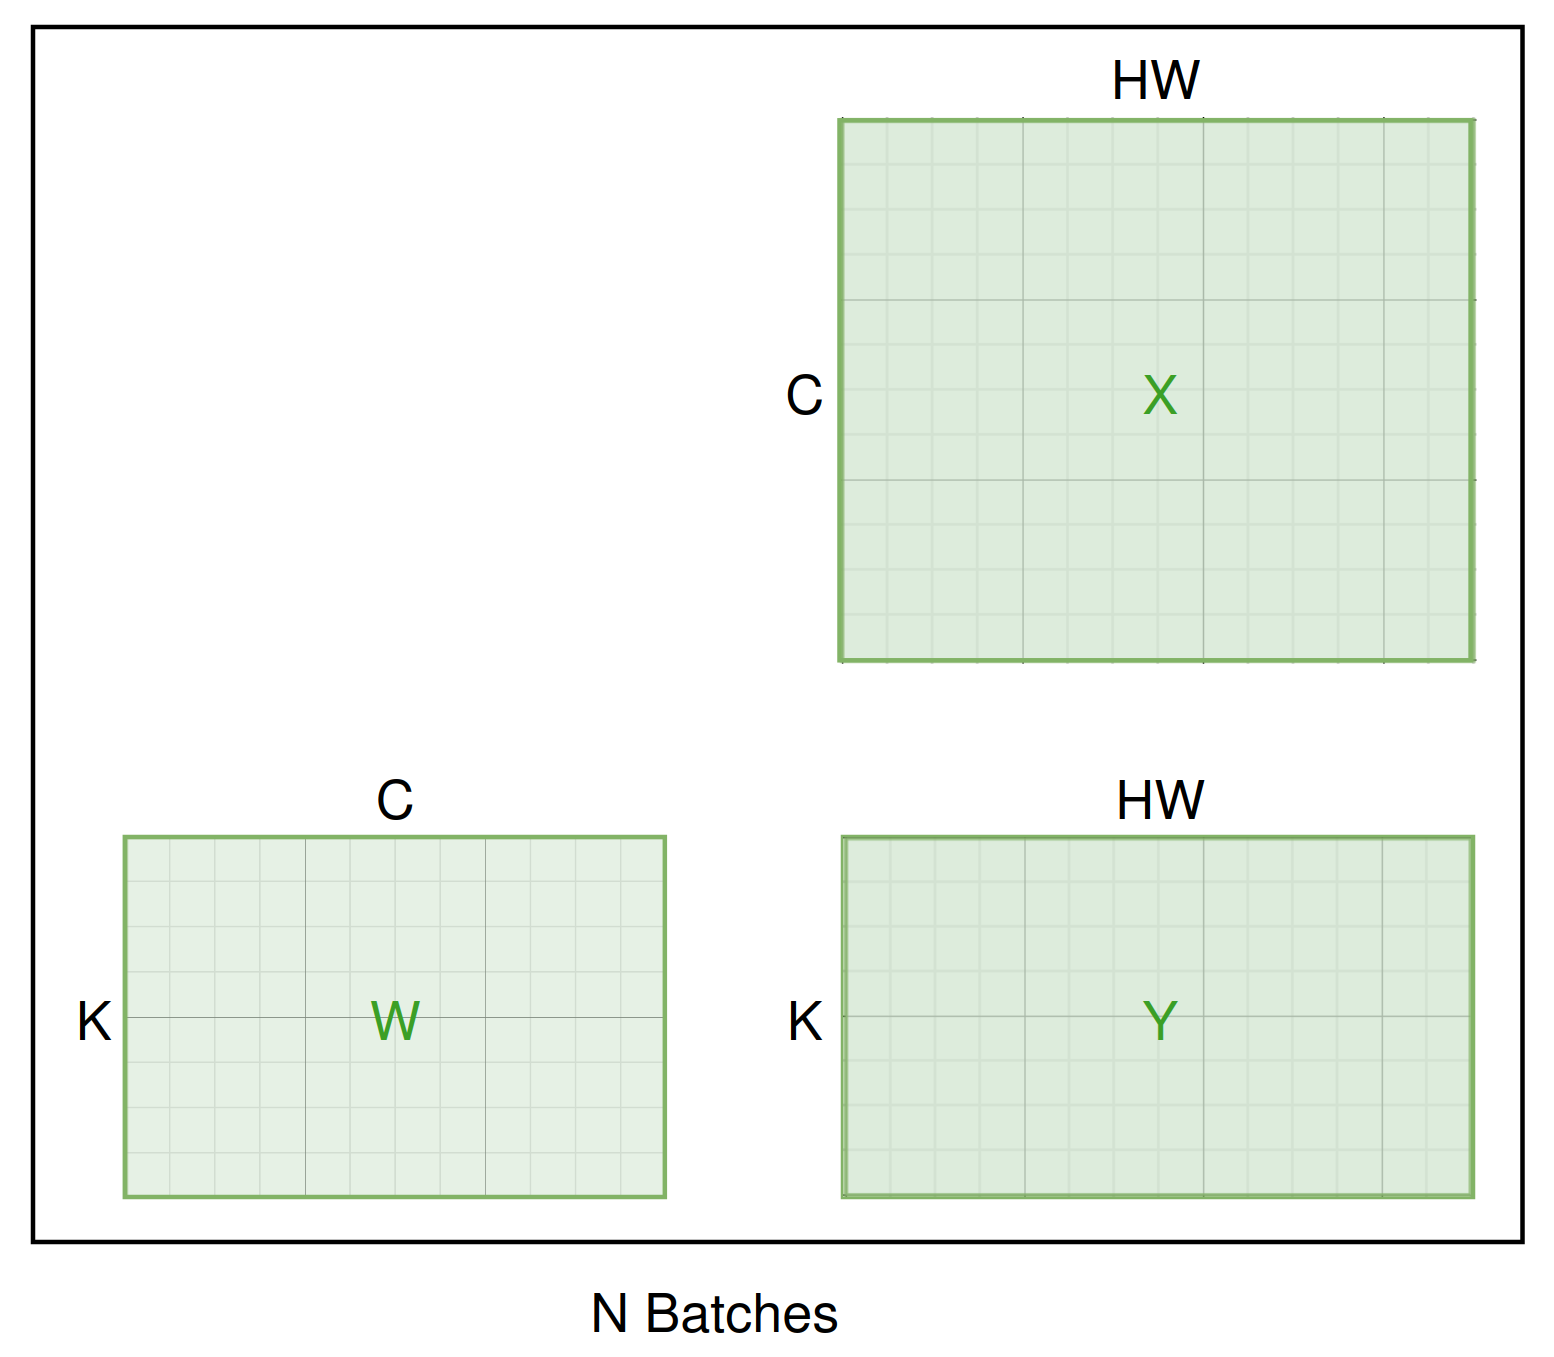
\includegraphics[width=0.8\textwidth]{src/images/1x1s0.png}
    \caption{Графическая схема преобразования свертки $1 \times 1$ с единичным шагом и нулевым дополнением в пакетное матричное умножение}
    \label{fig:1x1s0}
\end{figure}

На рисунке \ref{fig:1x1s0} показана визуализация данного преобразования, демонстрирующая эквивалентность операции свертки и пакетного матричного умножения.
Такое представление особенно полезно для оптимизации реализации, так как позволяет применять высокоэффективные алгоритмы матричного умножения, реализованные
в библиотеке CUTLASS.

\begin{figure}[h]
    \centering
    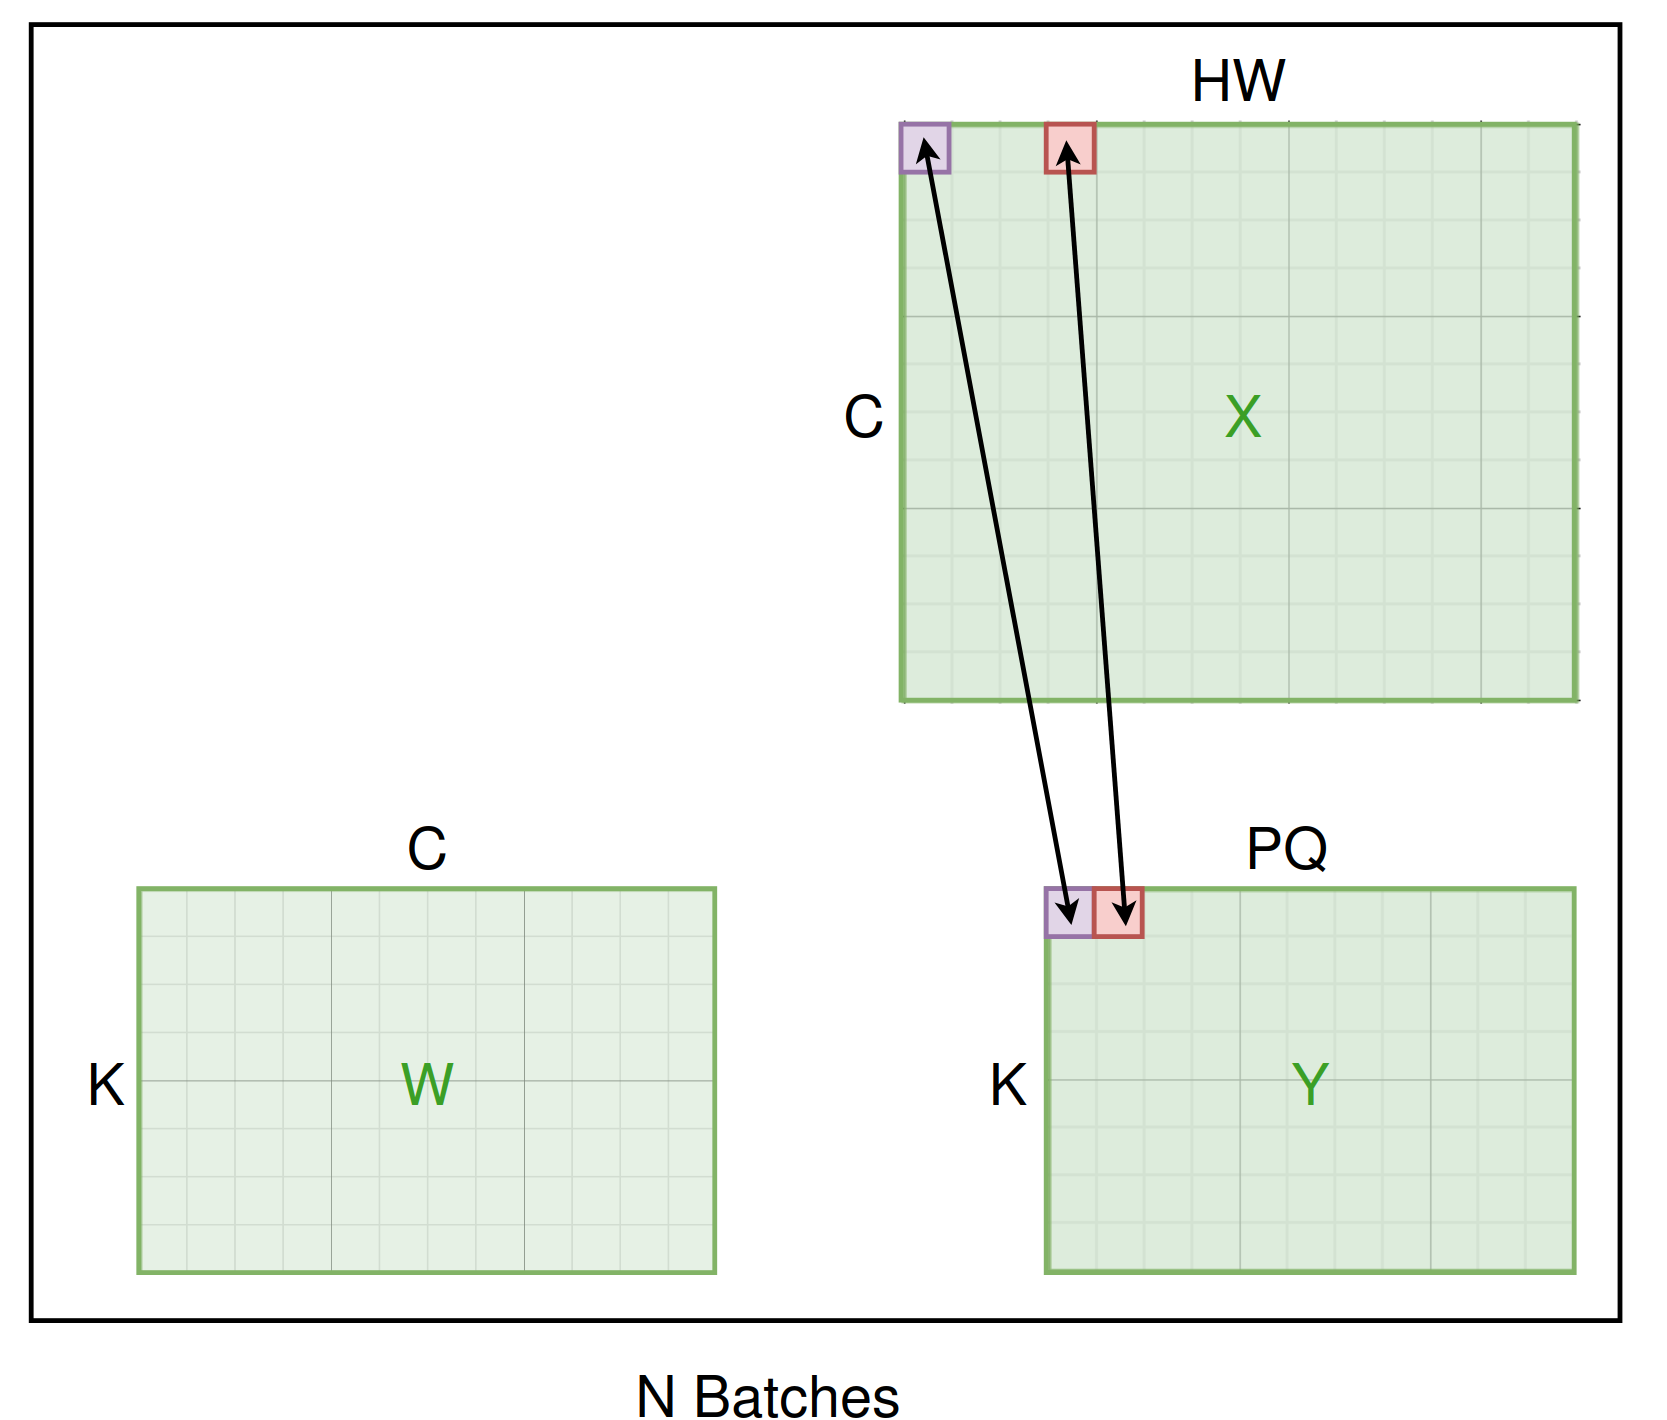
\includegraphics[width=0.8\textwidth]{src/images/1x1sn.png}
    \caption{Графическая схема преобразования свертки $1 \times 1$ с произвольным шагом и нулевым дополнением в пакетное матричное умножение}
    \label{fig:1x1sn}
\end{figure}

В случае свертки с произвольным шагом необходимо внести изменения в алгоритм пакетного матричного умножения.
Координаты входного тензора определяются соотношениями $\bar{h} = p \cdot s_h$ и $\bar{w} = q \cdot s_w$, где $s_h$ и $s_w$ — шаги свертки по
высоте и ширине соответственно.

Алгоритм преобразования включает следующие этапы:
\begin{enumerate}
    \item Введение составного индекса выходных пространственных координат: $pq = p \cdot Q + q$,
    \item Восстановление координат: $p = \lfloor pq / Q \rfloor$, $q = pq \bmod Q$,
    \item Вычисление соответствующих координат входного тензора: $\bar{h} = p \cdot s_h$, $\bar{w} = q \cdot s_w$.
\end{enumerate}

С математической точки зрения операция свертки записывается как

\begin{equation}
y[n, k, pq] = \sum_{c=0}^{C-1} w[k, c] \cdot x[n, c, \bar{h}\bar{w}],
\end{equation}

где индекс $\bar{h}\bar{w} = \bar{h} \cdot W + \bar{w}$ — линеаризованный индекс входного тензора.

Визуализация данного алгоритма приведена на рисунке \ref{fig:1x1sn}.

Оптимизированная реализация достигла 100 \% среднегеометрической производительности относительно cuDNN для
шага 1 и 85 \% для шага $>1$ (Рис. \ref{fig:conv1x1_res}):

\begin{figure}[htbp]
\centering
\begin{tikzpicture}
\begin{axis}[
    ybar=0pt,
    bar width=15pt,
    width=8cm,
    height=6cm,
    ylabel={Производительность относительно cuDNN},
    xlabel={Тип свёртки},
    symbolic x coords={k1x1s1x1, k1x1s2x2},
    xtick=data,
    xticklabel style={rotate=45, anchor=east},
    ymin=0,
    ymax=1.4,
    enlarge x limits=0.5,
    legend style={
        at={(0.5,1.03)},
        anchor=south,
        legend columns=-1,
    },
    nodes near coords,
    nodes near coords align={vertical},
    grid=major,
    grid style={dashed,gray!30}
]
\addplot+[
    style={fill=blue!40},
    every node near coord/.append style={
        font=\scriptsize,
        anchor=south
    }
] coordinates {(k1x1s1x1,1.0) (k1x1s2x2,0.85)};

\addplot+[
    style={fill=red!50},
    every node near coord/.append style={
        font=\scriptsize,
        anchor=south,
        xshift=4pt,
    }
] coordinates {(k1x1s1x1,0.56) (k1x1s2x2,0.62)};

\legend{Оптимизированный, Базовый}
\end{axis}
\end{tikzpicture}
\caption{Сравнение среднегеометрической производительности реализации свертки 1x1 для формата
NCHW относительно cuDNN: до оптимизации и после}
\label{fig:conv1x1_res}
\end{figure}

TBD;